\chapter{Software Architecture }
The resource management system has a client-server-based software architecture. In this architecture, the client application is used by the administrators and other end-users. The client sends requests to the server using GraphQL. The server validates the client and their request, queries the database, does some computation and sends the response to the client.
\section{Technical Stack}
\subsection{Angular}
Angular is a modern front end web development framework built by Google. It is a component based framework for scalable web applications with well-integrated libraries that covers a wide range of features like routing, client-server communication, etc. A complementary package of UI components for Angular is PrimeNG. PrimeNG has over 90 components, with variety of themes, and templates to build a responsive web application. 

\subsection{APIs}

The application programming interface (API) is a intermediate software that facilitates communication between the client and the server. Resource Management System uses GraphQL for server communication and REST API for third party services. 

GraphQL is a data query/manipulation language developed by Facebook. The main advantage of GraphQL over REST API is avoid under-fetching and over-fetching. GraphQL provides exactly the required content to render the with exactly one API end point and one request. The Apollo GraphQL is a software platform that immensely simplifies the underlying complexity, and unifies GraphQL across multiple apps.

The third party service used is Google Custom Search Engine (CSE). This service provides a REST API endpoint, using which we can query to get result from the web. Resource management system uses Google CSE to get images for facilities, categories, and items to suggest during its creation. 

\subsection{NestJS}
NestJS is a progressive Node.js framework for developing effective, scalable and reliable server-side applications. It uses the latest JavaScript features, and design patterns. NestJS provides various wrapper libraries for popularly used packages such as apollo-graphql, JWT authentication, etc. 

\subsection{Database}
Resource management system uses MongoDB which is a No-SQL database built for handling big data related tasks more efficiently. Some advantages of MongoDB over SQL databases are:
\begin{itemize}
    \item It has a very flexible schema which allows us to evolve and store data easily.
    \item Apart from supporting all features of relational databases, it is built to scale up much faster.
    \item MongoDB schemas are more intuitive to developers using JS based languages and since our technical stack is completely works by handling JSON data, using MongoDB is a more appropriate choice.
\end{itemize}

\begin{figure}[H]
    \centering
    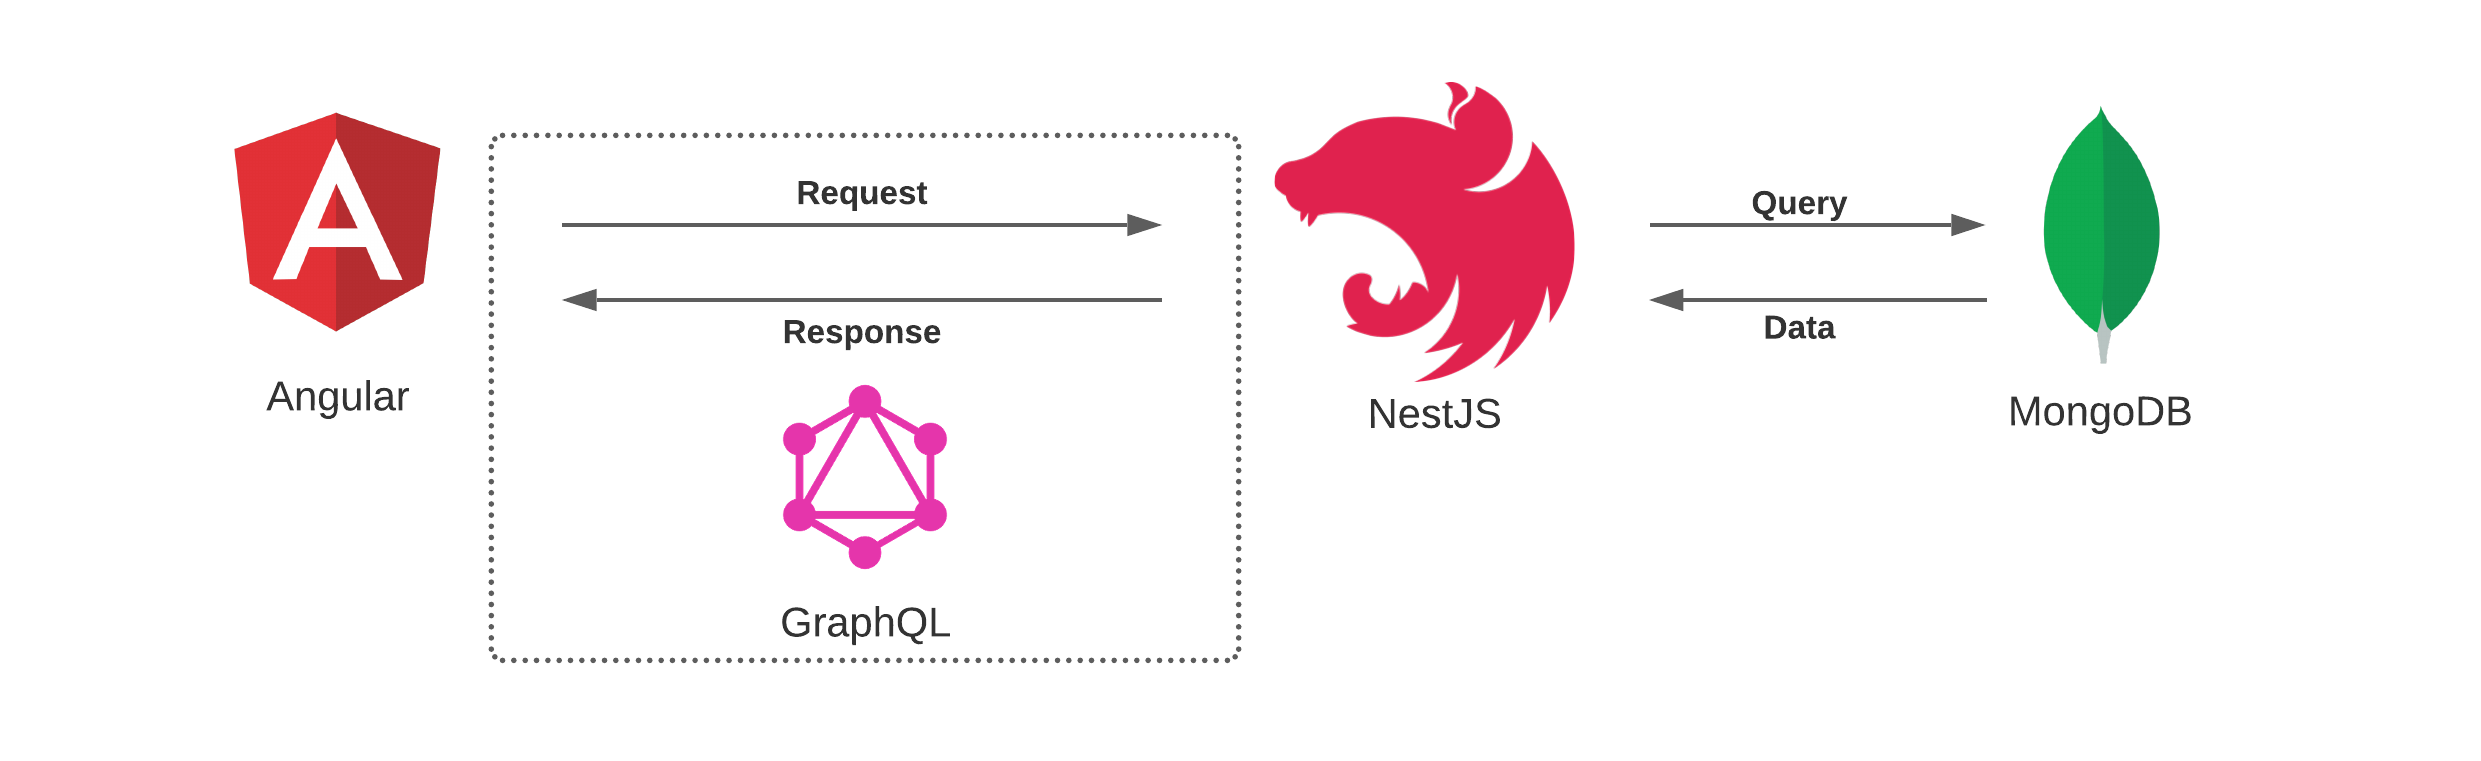
\includegraphics[scale=0.15]{images/tech-stack.png}
    \caption{Complete technical flow}
    \label{fig:tech-stack}
\end{figure}

\subsection{Development tools}
\begin{itemize}
    \item \textbf{Docker}: It allows developers to work and deploy apps without being concerned about the various dependencies needed.
    \item \textbf{GitHub}: It is used for version control and collaboration.
    \item \textbf{Figma}: It is an vector graphics UI designing programs.
    \item \textbf{Postman}: It is a platform to test, build and share APIs. It simplifies API life-cycle and collaboration.
\end{itemize}

\begin{minted}{gql.py:GraphqlLexer -x}
mutation updateCheckoutShippingOptions(
  $checkoutId: ID!
  $shippingMethodId: ID!
) {
  checkoutShippingMethodUpdate(
    checkoutId: $checkoutId
    shippingMethodId: $shippingMethodId
  ) {
    errors {
      field
      message
      __typename
    }
    checkout {
      ...Checkout
      __typename
    }
    __typename
  }
}
\end{minted}